\clearpage
\chapter{Background Estimation}\label{sec:estimate}

Section ~\ref{sec:selections} listed several different discriminant variables for the analysis.
Leading ROI vertex score, subleading ROI vertex score, and leading muon's IP value have the most discriminatory power.
Although the background MC samples describe the data's distribution fairly well, one can also see discrepancy at higher vertex score and higher IPSig values.
This originates from 2 different reasons.
First, the lack of statistics is a fundamental deficiency for the MC samples.
Unlike 11.9 billion events b-parking data, MC sample events are simulated with extremely intensive computing resources.
Thus, its event number is limited below 100 milion at most, failing to describe distributions for extreme values.
Second, the QCD MC's data description accuracy lacks compared to other physics process.
QCD background, which is the main background for the analysis, is a quantum-chromodynamics process.
QCD involves a lot of uncertainty and relies on probablistic description at low energy.
Therefore, QCD's description accuracy lacks compared to other process such as WJets and Drell-Yan process.
Since MC does not describe the data in a satisfactory manner, the analysis uses data-driven background estimation method.


\section{ABCD method}
For any background estimation method, ABCD method is the most preferred thanks to its simplicity.
ABCD method is a simplest form of transfer-factor.
A ratio of background event at 2 control region (CR) is applied to another CR's background event to infer background event in signal region (SR) without unblinding.
Simplest mathematical for is described in formula \ref{eq:ABCD}.
\begin{equation}
\label{eq:ABCD}
	SR:CR1=CR2:CR3, SR=CR1*\frac{CR2}{CR3} 
\end{equation}
ABCD method requires 2 variables used for its estimation should be independent of each other for background process.


Unfortunately, leading ROI vertex score and subleading ROI vertex score are correlated in the QCD background process.
ROIs from B-mesons score higher in our tensorflow.
In QCD processes, the B-mesons are likely to be pair produced.
Therefore, when the leading ROI vertex score is high due to its b-like behavior, the sublead ROI vertex score is also high because the anti-meson is produced on the other side of the detector.
Thus, leading and sublead scores can't be our ABCD discriminant variable candidates due to their correlation.

The analysis selects leading ROI and leading muon's IP value as its ABCD discriminant variables.
After implementing all other cuts (sublead ROI, $\Delta\Phi(lead,sublead)$, Annulus score, 1 Isolated $\mu$, $\Delta R(lead ROI, Jet)$), we tested the correlation factor between the leading ROI, and leading mu's IPSig values for each background process.
The values are pretty minimal except for 2-3 processes where there were too few entries to derive a physical conclusion due to statistical limitations.
Therefore, the analysis uses leading Log10(IPSig) and leading ROI vertex score for its ABCD discriminant variables.

The results are listed below.  


 \begin{figure}[h!]
   \caption{Cutflow histogram of MS15GeV-ct100mm point. Left plot is for region A, whereas the right plot is for region D}
   \label{fig:ABmethod}
   \centering
   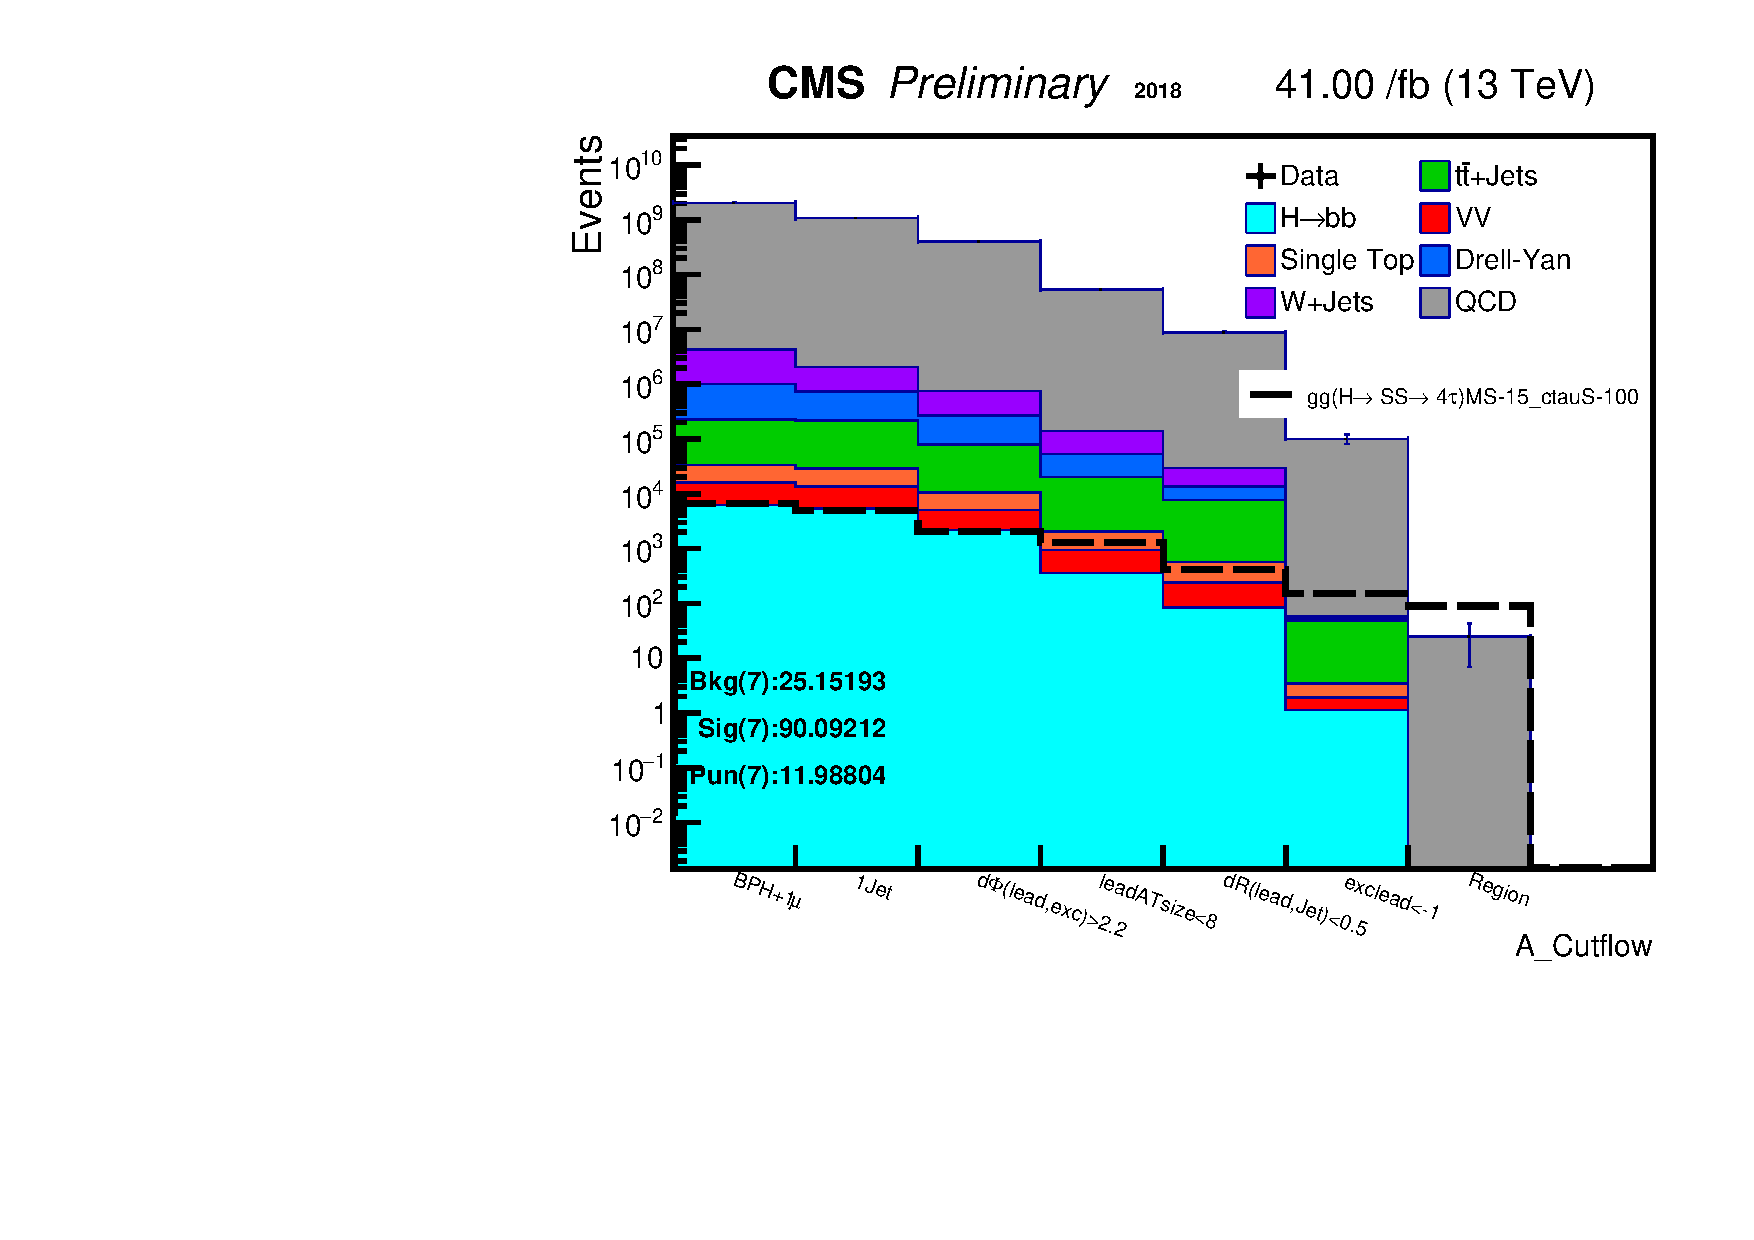
\includegraphics[width=0.47\linewidth]{figs/AnalysisNoteplot_MS-15_ctauS-100_A_Cutflow.pdf}
   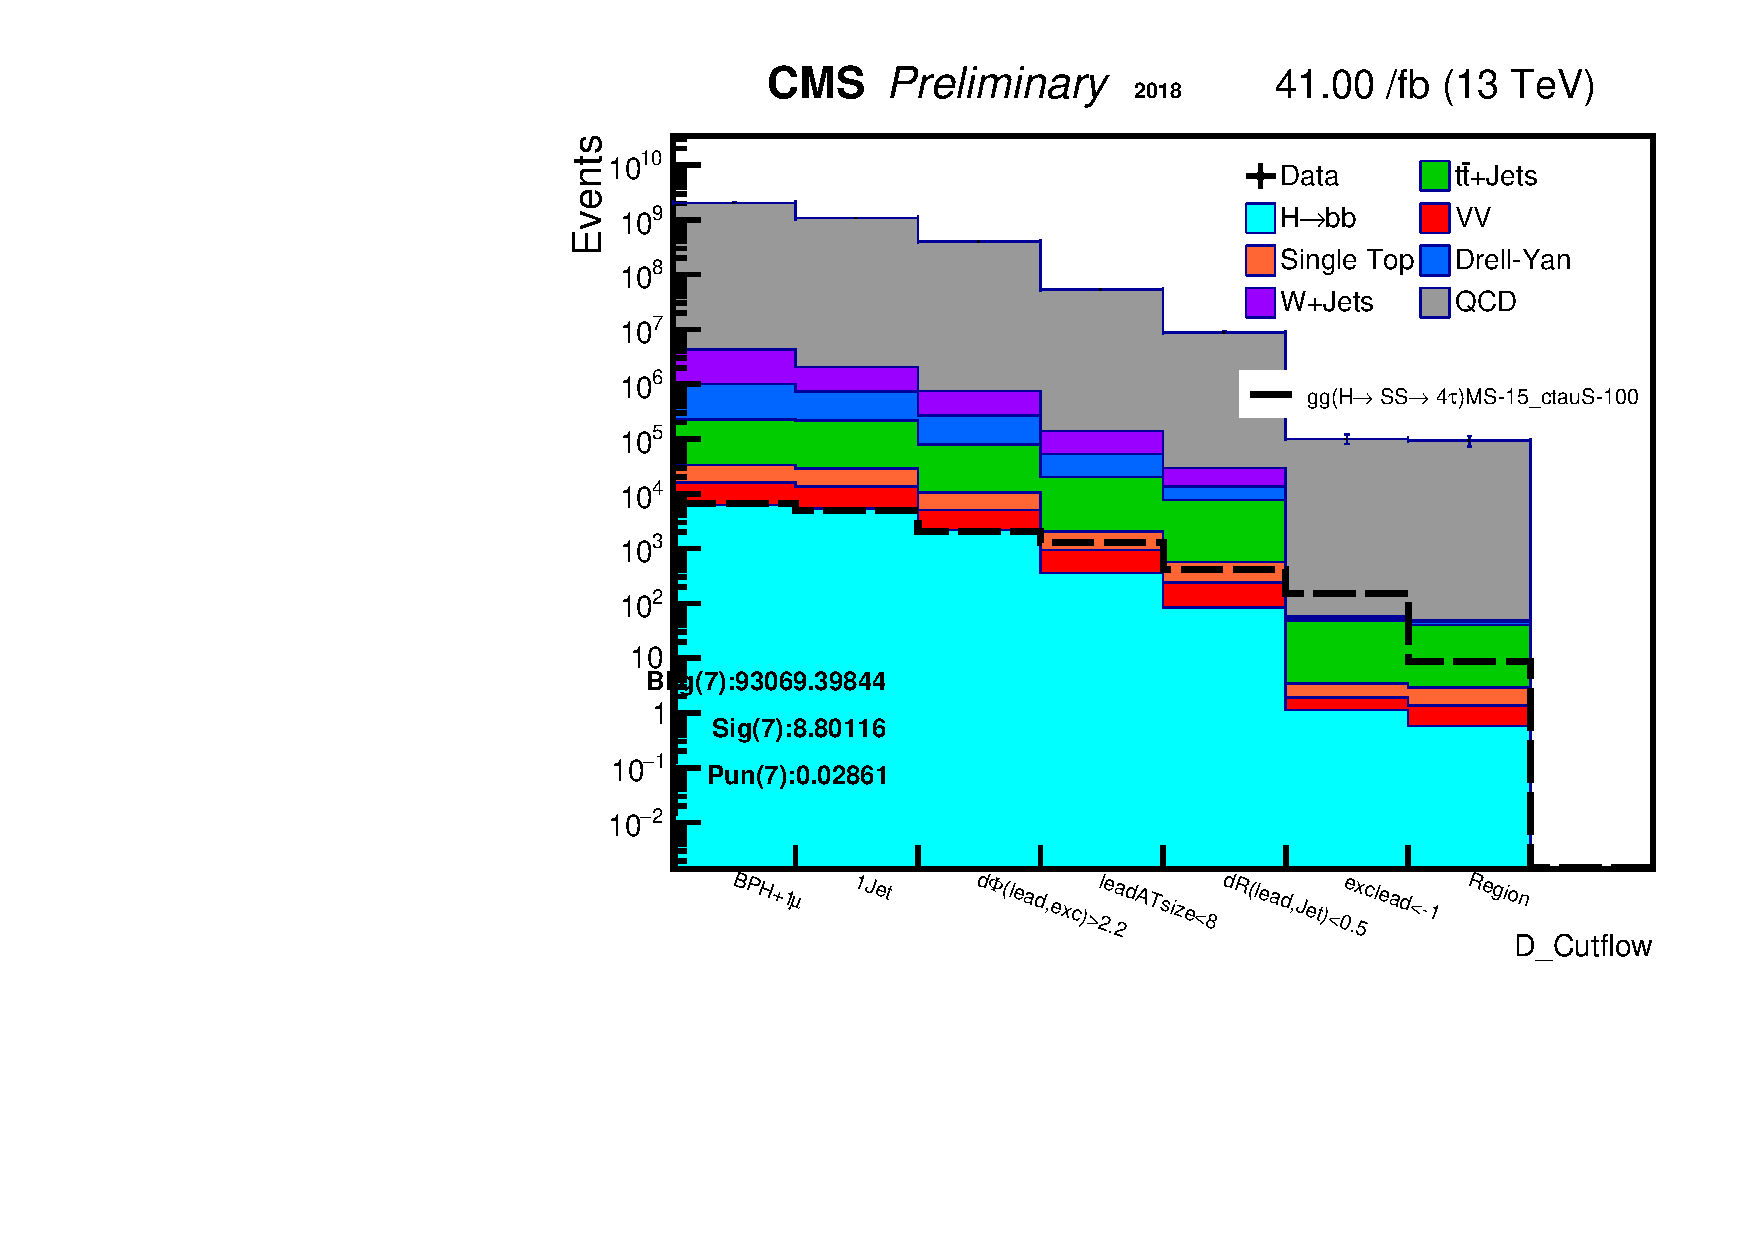
\includegraphics[width=0.47\linewidth]{figs/AnalysisNoteplot_MS-15_ctauS-100_D_Cutflow.pdf}
 \end{figure}

 \begin{figure}[h!]
   \caption{eee}
   \label{fig:ABCDmethod}
   \centering
   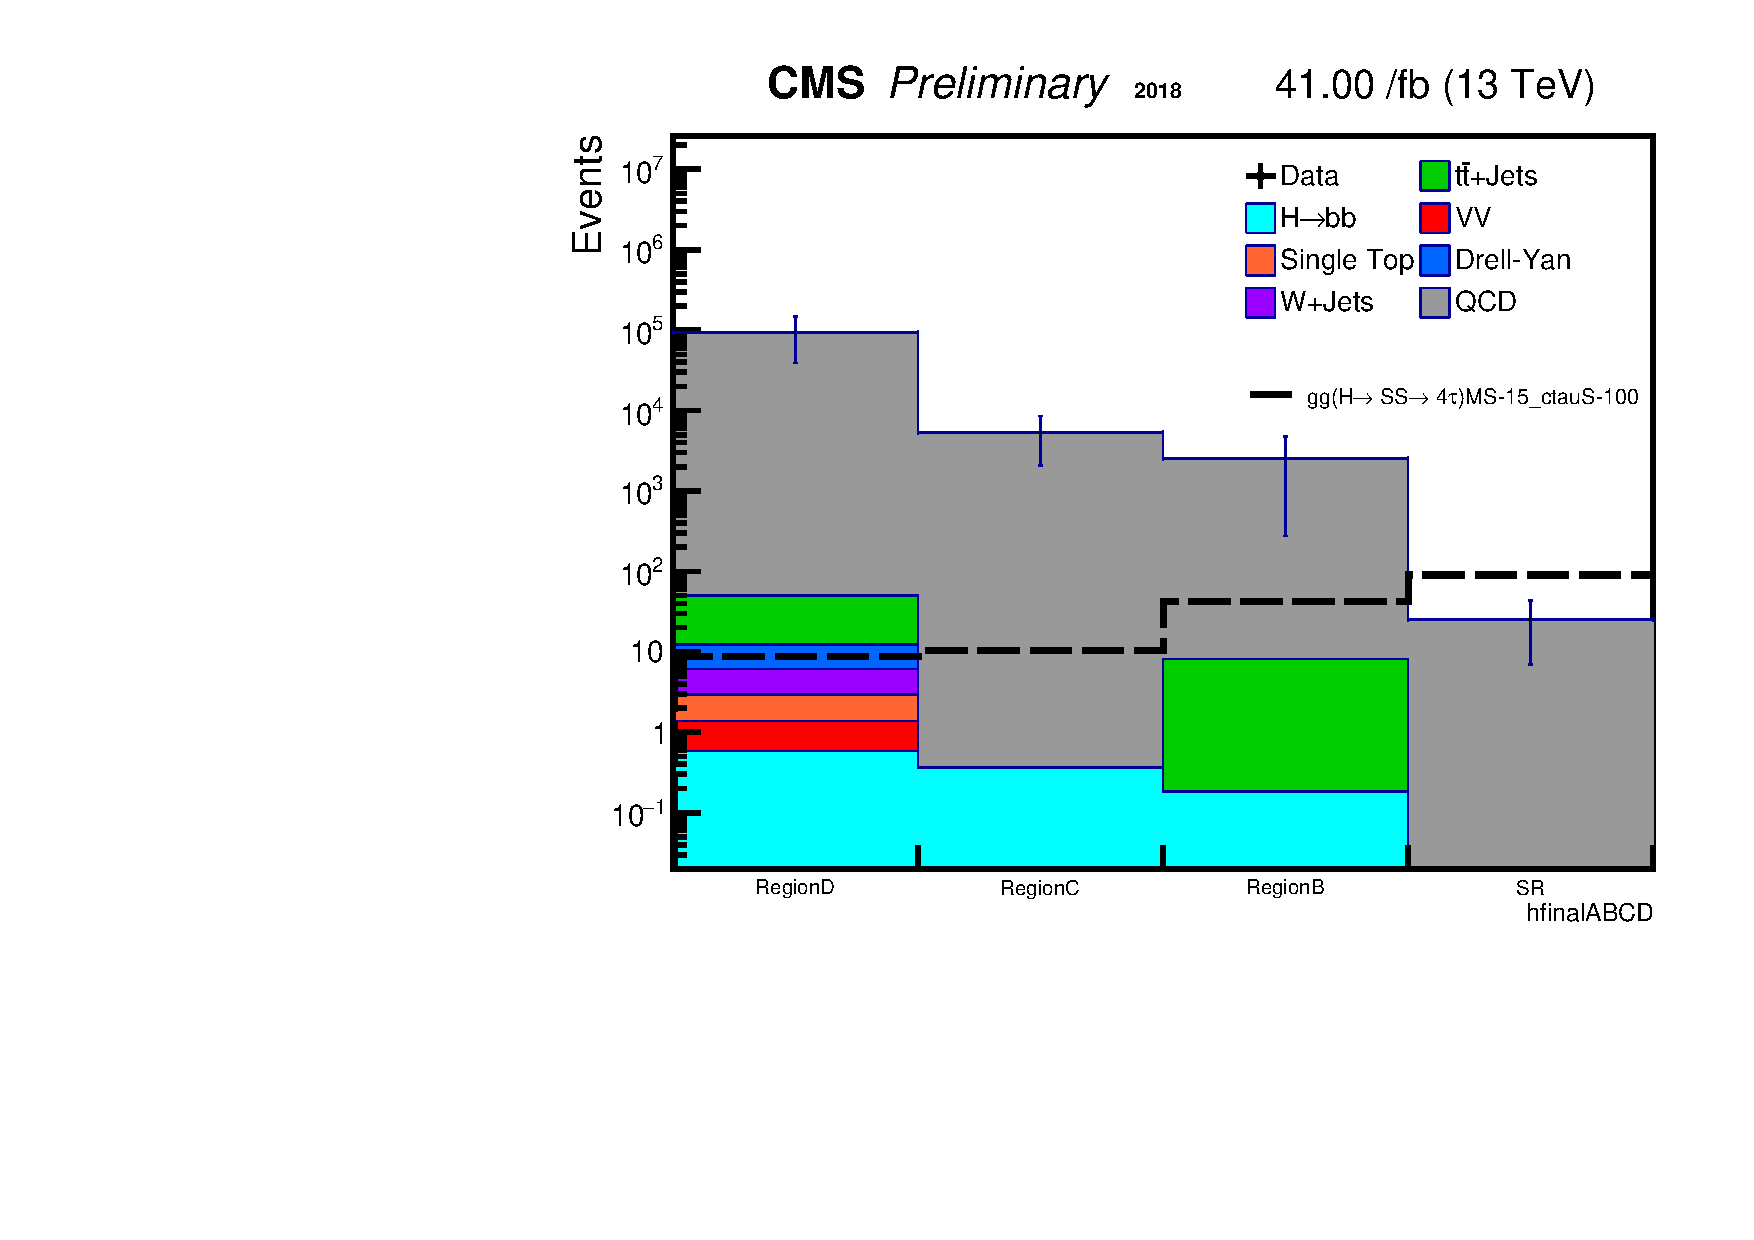
\includegraphics[width=0.67\linewidth]{figs/AnalysisNoteplot_MS-15_ctauS-100_hfinalABCD.pdf}
 \end{figure}

\section{Validation of ABCD method}

Although background MC's correlation factor($\^{r}$) values are small, we need to verify that the data's correlation factor is negligible since data will be used for our background estimation.
However, direct computation of $\^{r}$(leadROI,Log10(muIPSig)) for data is problematic because the CMS community stipulates "blinding".
In general, high signal ratio is expected in singal region.
In order to avoid bias for new discovery and changing their analysis strategy, the CMS recommends physicists to blind themselves from looking into data entry in the signal region, until community acknowledgement is granted.
This concept is called "blinding"
Since one can not have access for data entry in the signal region, data's correlation factor($\^{r}$) can not be computed. 
Therefore, one needs to find an alternative way to estimate data's $\^{r}$(leadROI,Log10(muIPSig)) without unblinding data in the signal region.

For this purpose, we define a new ABCD region, referred to as A'B'C'D'.
A'-D' region is an orthogonal plane to the original ABCD, where the d$\phi$ category of the event selection is flipped while all other event selection cuts are removed.
Region A', a correspondant Signal region of the orthogonal plane, should be much lower in signal ratio (background dominated): Only so, looking into data entry in A' is not problematic. 
In figures of a-b, we confirm that background dominates the A' region while the signal entry is lower regardeless of the signal's MS and ctau.





In A'-D' region, we can see the correlation factor is about 10\%, still a negligible value. 


With $\^{r}$(leadROI,Log10(muIPSig)) value in A'-D' region, It seems sufficient to claim that there should be negligible correlation between leadROI and Log10(muIPSig) for A-D region as well.
Unfortunately, suspicious people could throw 1 last question.
What if $\^{r}$(leadROI,Log10(muIPSig)) value changes with respect to d$\phi$?
If the formula in \ref{eq:rhat} is not true, $\^{r}$(leadROI,Log10(muIPSig)) obtained from A'-D' is not a good estimate for $\^{r}$(leadROI,Log10(muIPSig)) for A-D.

To check that formula \ref{eq:rhat} is true, we subdivide A'-D'.
A1'-D1' are orthogonal planes where d$\phi$ is closest to A-D.
Increasing numeric value indicates how far the d$\phi$ is from the A-D.
$\^{r}$(leadROI,Log10(muIPSig)) value for each of A'-D' region is plotted in figures and summarized in table.



As we scan $\^{r}$(leadROI,Log10(muIPSig)) for each d$\phi$ section, very small trend with respect to d$\phi$ is observed.
We can claim the formula \ref{eq:rhat} is true and $\^{r}$(leadROI,Log10(muIPSig)) from A'-D' can be translated into A-D region as well.


Since there is not correlation of 2 variables for ABCD region, we validated the background estimation method.
With background rate in signal region estimated by ABCD method with data, and with signal MC, we can either claim there exists signal over the SM expectation or not.
If it does not, we can claim an exclusion limit on the branching ratio of the signal to a certain value.


Before that systematics



